% Chapter 4: Methodology
\chapter{Methodology}

This chapter presents the comprehensive methodology used in the development of the Timetable Buddy system. It includes various modeling diagrams, project management artifacts, and quality assurance documentation that guided the systematic development approach for creating a robust lecture scheduling solution.

\section{Data Flow Diagrams (DFD)}

Data Flow Diagrams represent the flow of data through the system at different levels of abstraction, showing how information moves between processes, data stores, and external entities in the Timetable Buddy system.

\subsection{DFD Level 0 (Context Diagram)}

The Context Diagram provides a high-level view of the entire Timetable Buddy system, showing its interaction with external entities including Students, Faculty, and Administrators.

\begin{figure}[htbp]
    \centering
    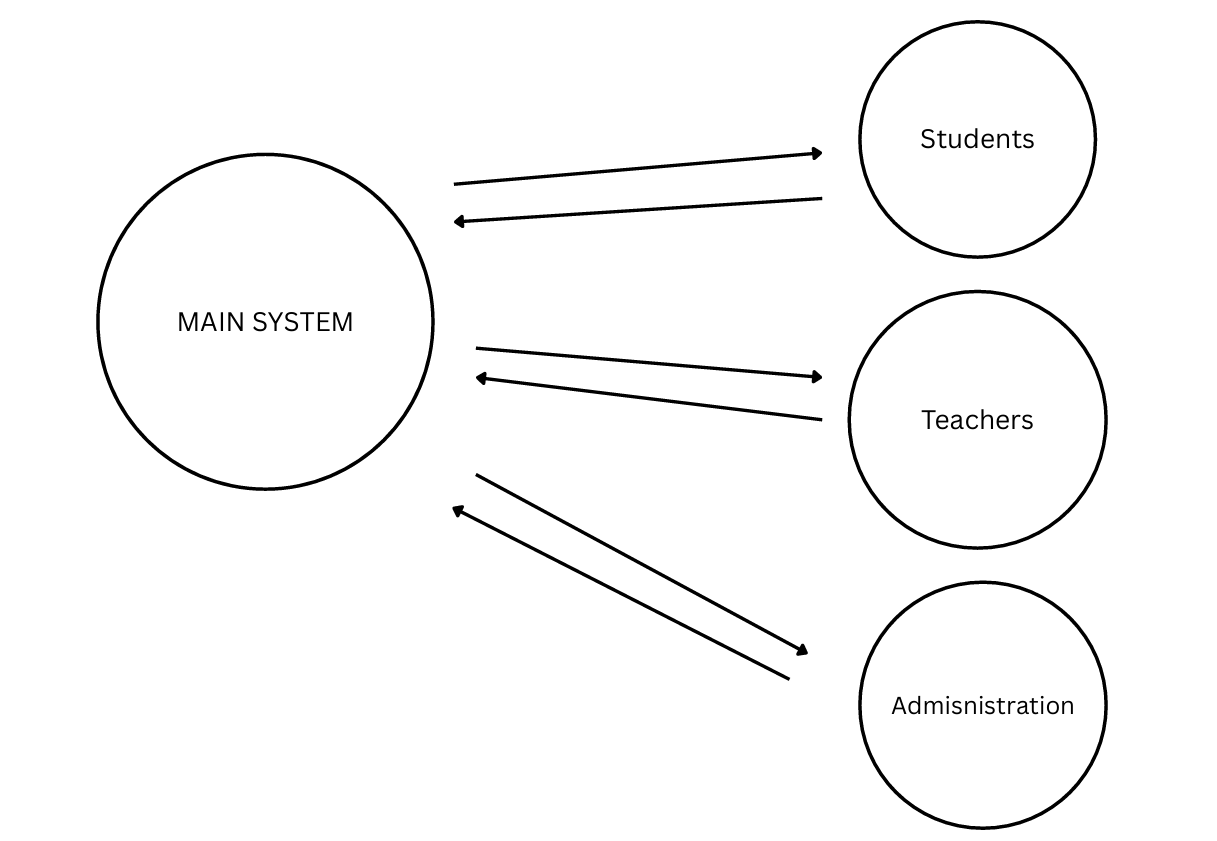
\includegraphics[width=0.85\textwidth]{images/DFD Level 0.png}
    \caption{DFD Level 0 - Context Diagram showing system boundaries and external entities}
    \label{fig:dfd0}
\end{figure}

The context diagram provides a comprehensive overview of the Timetable Buddy system's interaction with its operational environment, clearly defining the boundaries between internal system processes and external entities. The diagram identifies three primary external entities that interact with the system: Students who utilize the platform for course enrollment and schedule management, Faculty members who create and manage lecture slots while monitoring student participation, and Administrators who oversee system-wide operations and maintain institutional policies. At the center of this diagram, the Timetable Buddy System serves as the central processing hub that orchestrates all interactions between these external entities and manages the complex data transformations required for effective academic scheduling. The data flows depicted in the diagram encompass authentication requests that verify user identities and establish secure sessions, enrollment data that captures student registration preferences and course participation, lecture schedules that define the temporal and spatial parameters of academic sessions, and comprehensive timetable information that provides consolidated views of academic activities. The system boundary clearly delineates between internal processes that occur within the Timetable Buddy platform and external interactions that involve human users or other institutional systems, ensuring that the scope and responsibilities of the scheduling system are precisely defined.

\subsection{DFD Level 1 (High-Level Processes)}

Level 1 DFD decomposes the main system into major processes, showing the primary functional components and their interactions with data stores and external entities.

\begin{figure}[htbp]
    \centering
    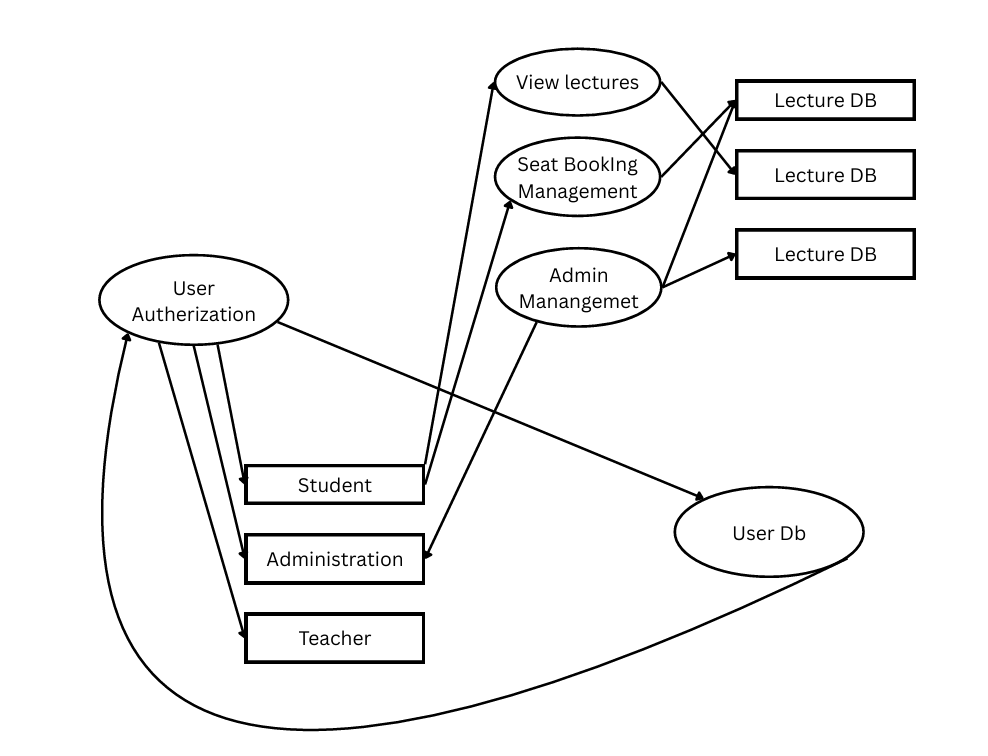
\includegraphics[width=0.95\textwidth]{images/DFD Level 1.png}
    \caption{DFD Level 1 - Major system processes and data stores}
    \label{fig:dfd1}
\end{figure}

The Level 1 Data Flow Diagram reveals the sophisticated internal architecture of the Timetable Buddy system through the identification of five critical processes that collectively deliver comprehensive academic scheduling functionality. Process 1 encompasses User Authentication and Authorization mechanisms that verify user identities, establish secure sessions, and implement role-based access controls that ensure appropriate system permissions for different user categories. Process 2 focuses on Lecture Slot Management operations that enable authorized users to create, modify, and maintain lecture slots while ensuring data integrity and proper scheduling coordination. Process 3 handles Enrollment Processing activities that manage student registrations, implement conflict detection algorithms, maintain waitlist functionality, and coordinate automatic promotion procedures when enrollment capacity changes occur. Process 4 involves Timetable Generation and Display operations that synthesize enrollment data and lecture slot information into coherent schedule presentations customized for different user roles and preferences. Process 5 encompasses Dashboard and Analytics functionality that provides users with personalized insights, statistical summaries, and operational metrics relevant to their academic scheduling activities. The diagram also identifies critical data stores that support these processes, including the User Database that maintains account information and authentication credentials, the Lecture Slots repository that stores course scheduling details and capacity information, the Enrollments database that tracks student registrations and waitlist positions, and the Schedules data store that preserves generated timetable configurations and historical scheduling patterns.

\subsection{DFD Level 2 (Detailed Processes)}

Level 2 DFD provides detailed decomposition of complex processes from Level 1, showing sub-processes and their detailed interactions within the enrollment management system.

\begin{figure}[htbp]
    \centering
    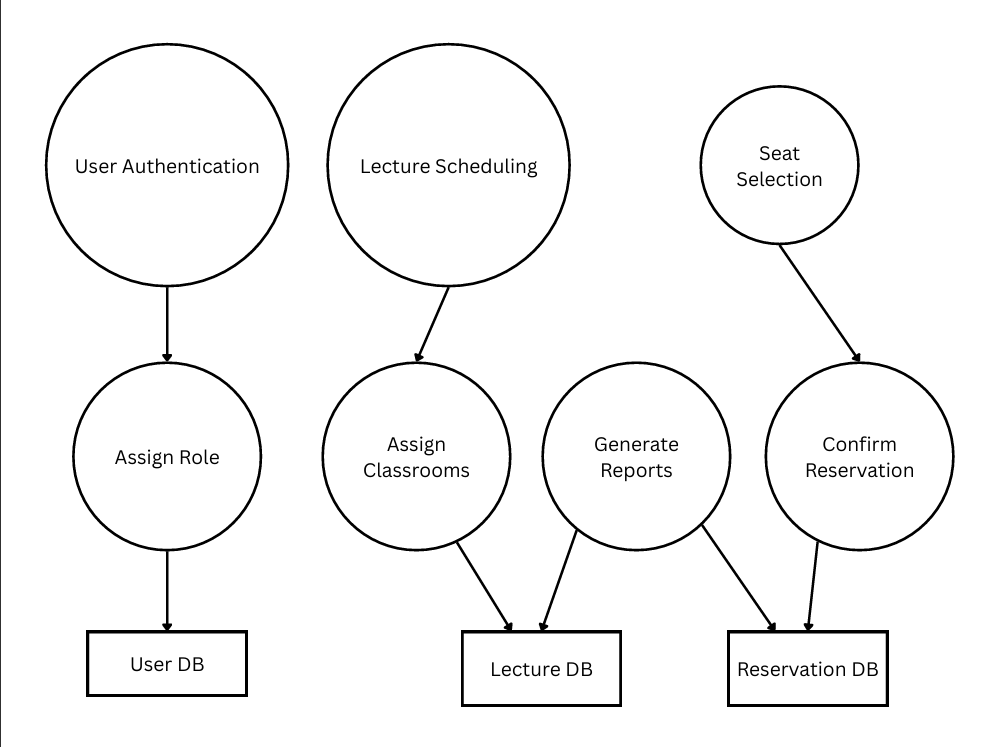
\includegraphics[width=0.95\textwidth]{images/DFD Level 2.png}
    \caption{DFD Level 2 - Detailed process decomposition}
    \label{fig:dfd2}
\end{figure}

The Level 2 Data Flow Diagram provides an intricate examination of the enrollment management subsystem, revealing the sophisticated sub-processes that orchestrate student course registration and academic schedule coordination. The enrollment workflow with waitlist management demonstrates how the system processes initial student registration requests, evaluates course capacity constraints, and seamlessly transitions students between active enrollment and waitlist positions based on availability and academic policies. The conflict detection mechanisms illustrate the complex algorithms that continuously monitor student schedules to identify potential time conflicts, prerequisite violations, or other academic constraints that might prevent successful course registration. Capacity validation processes showcase how the system maintains real-time awareness of course enrollment limits, manages overflow situations through waitlist functionality, and ensures that lecture slots never exceed their designated capacity while optimizing resource utilization. The notification generation sub-processes demonstrate how the system maintains continuous communication with students and faculty through automated messaging systems that provide updates about enrollment status changes, course modifications, and other relevant academic information that affects scheduling decisions.

\section{Use Case Diagram}

The Use Case Diagram illustrates the functional requirements from the user's perspective, showing the interactions between different actors and the system use cases.

\begin{figure}[htbp]
    \centering
    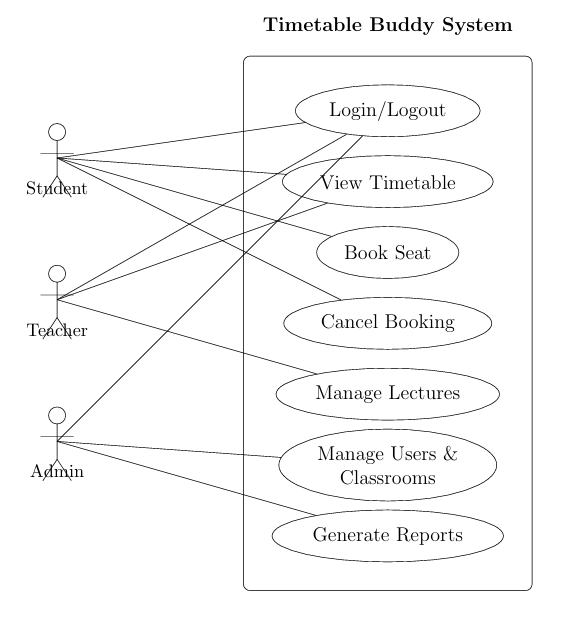
\includegraphics[width=0.85\textwidth]{images/Usecase diagram.png}
    \caption{Use Case Diagram showing actor interactions and system use cases}
    \label{fig:usecase}
\end{figure}

The Use Case Diagram identifies three primary actors who interact with the Timetable Buddy system, each possessing distinct responsibilities and access privileges that align with their institutional roles and academic responsibilities.

Students represent the primary user category within the system, possessing comprehensive capabilities that enable them to effectively manage their academic schedules and course enrollments. These users can access personalized timetable views that display their enrolled courses in intuitive calendar formats, facilitating effective time management and academic planning. Students utilize sophisticated enrollment functionality that allows them to register for available courses while benefiting from automatic conflict detection and waitlist management features. Profile management capabilities enable students to maintain current personal information, academic credentials, and communication preferences, ensuring that their system interactions remain personalized and effective. Additionally, students can monitor their enrollment status across all registered courses, providing transparency in their academic progress and enabling informed decisions about future course selections.

Faculty members operate within an expanded set of system capabilities that reflect their instructional responsibilities and course management needs. These users possess comprehensive lecture slot management functionality that enables them to create new courses, modify existing offerings, and maintain accurate scheduling information throughout academic terms. Faculty can access detailed enrollment information for their courses, including student contact details, participation statistics, and waitlist management tools that support effective course administration. Course detail management capabilities allow faculty to update syllabi, modify capacity limits, adjust scheduling parameters, and communicate important information to enrolled students through integrated messaging systems.

Administrators function at the highest privilege level within the system, possessing comprehensive oversight capabilities that support institutional management and strategic planning activities. These users maintain complete user management functionality that enables them to create, modify, and deactivate accounts for students, faculty, and other administrators while ensuring appropriate access controls and security measures. Course and lecture slot management capabilities provide administrators with system-wide visibility and control over academic offerings, enabling them to coordinate institutional scheduling policies and resolve conflicts that span multiple departments or programs. Advanced reporting functionality provides administrators with comprehensive analytics about system utilization, enrollment trends, resource allocation, and operational efficiency metrics that support data-driven decision making and strategic planning initiatives.

The system encompasses several critical use cases that define the core functionality available to these various actors. User authentication processes ensure secure access through comprehensive login and logout procedures that maintain session security while providing seamless user experiences. Lecture slot management operations enable authorized users to create, modify, and maintain course offerings while ensuring scheduling coordination and resource optimization. Course enrollment functionality provides students with intuitive registration processes that include conflict detection, waitlist management, and automatic notification systems. Timetable viewing capabilities deliver personalized schedule presentations that accommodate different user roles and preferences while maintaining data accuracy and real-time updates. Enrollment management tools provide faculty and administrators with comprehensive oversight of student registrations, waitlist positions, and course capacity utilization. Report generation functionality enables administrators to extract operational data, analyze system performance, and generate insights that support institutional planning and academic policy development.

\section{Sequence Diagram}

Sequence Diagrams show the interaction between objects over time, illustrating the message flow and order of operations for specific scenarios.

\begin{figure}[htbp]
    \centering
    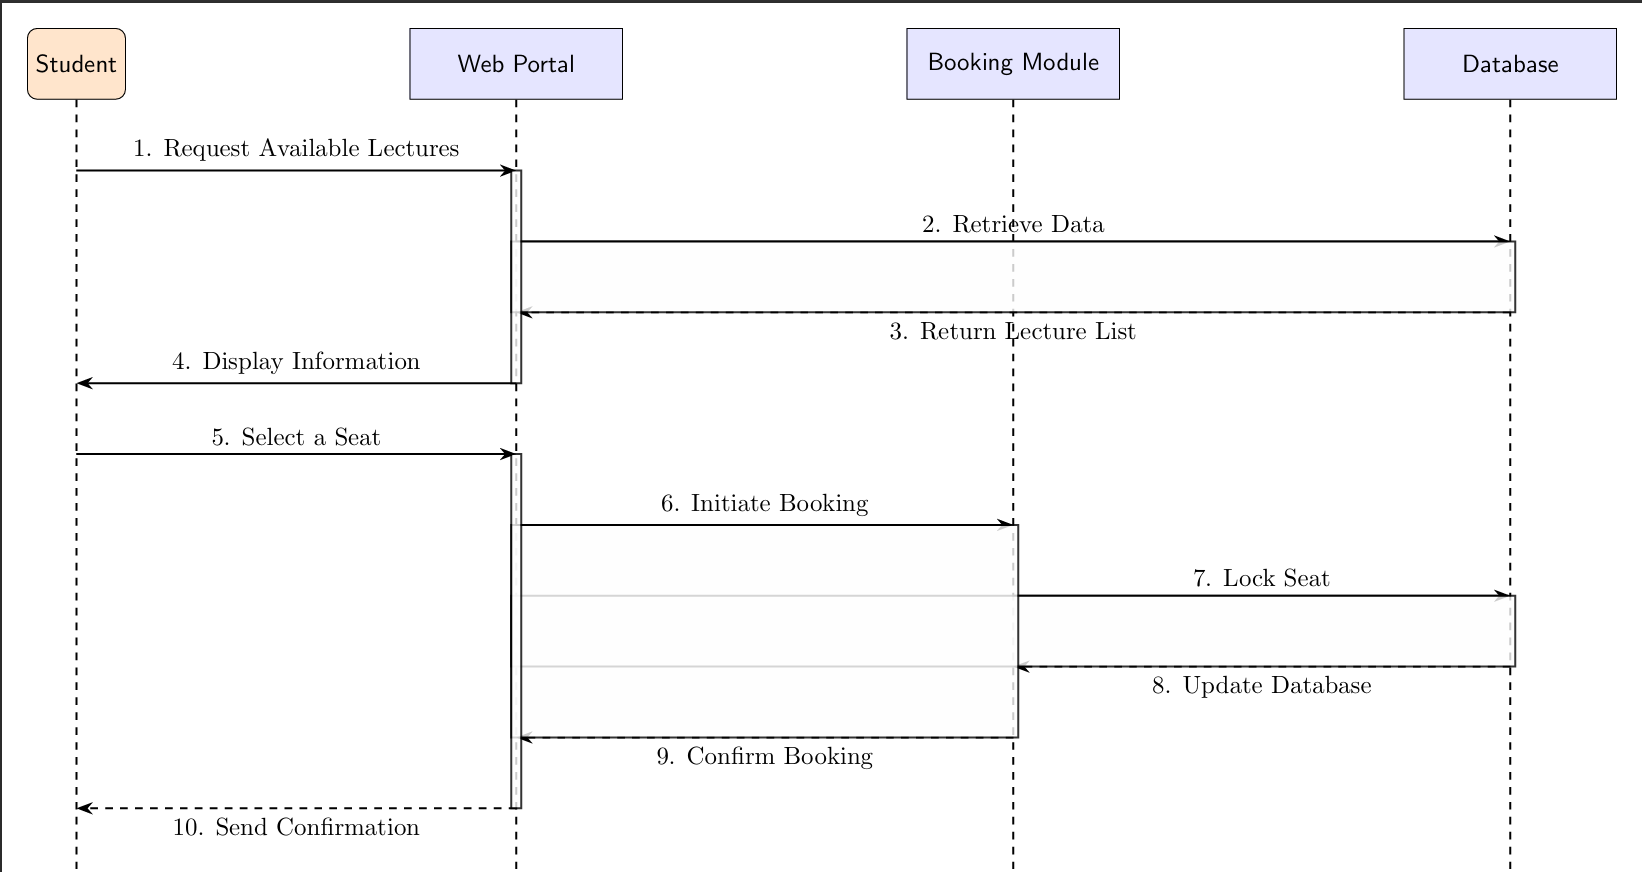
\includegraphics[width=0.9\textwidth,height=0.7\textheight,keepaspectratio]{images/Sequence Diagram.png}
    \caption{Sequence Diagram showing object interactions for enrollment process}
    \label{fig:sequence}
\end{figure}

The sequence diagram depicts:
\begin{itemize}[leftmargin=*]
    \item User authentication flow
    \item Enrollment request processing
    \item Conflict detection validation
    \item Capacity checking
    \item Database operations
    \item Response generation
\end{itemize}

\section{Activity Diagram}

Activity Diagrams model the workflow and business logic, showing the sequence of activities and decision points in system processes. The activity diagram provides a comprehensive view of the system's dynamic behavior, particularly focusing on the enrollment workflow and decision-making processes.

\begin{figure}[H]
    \centering
    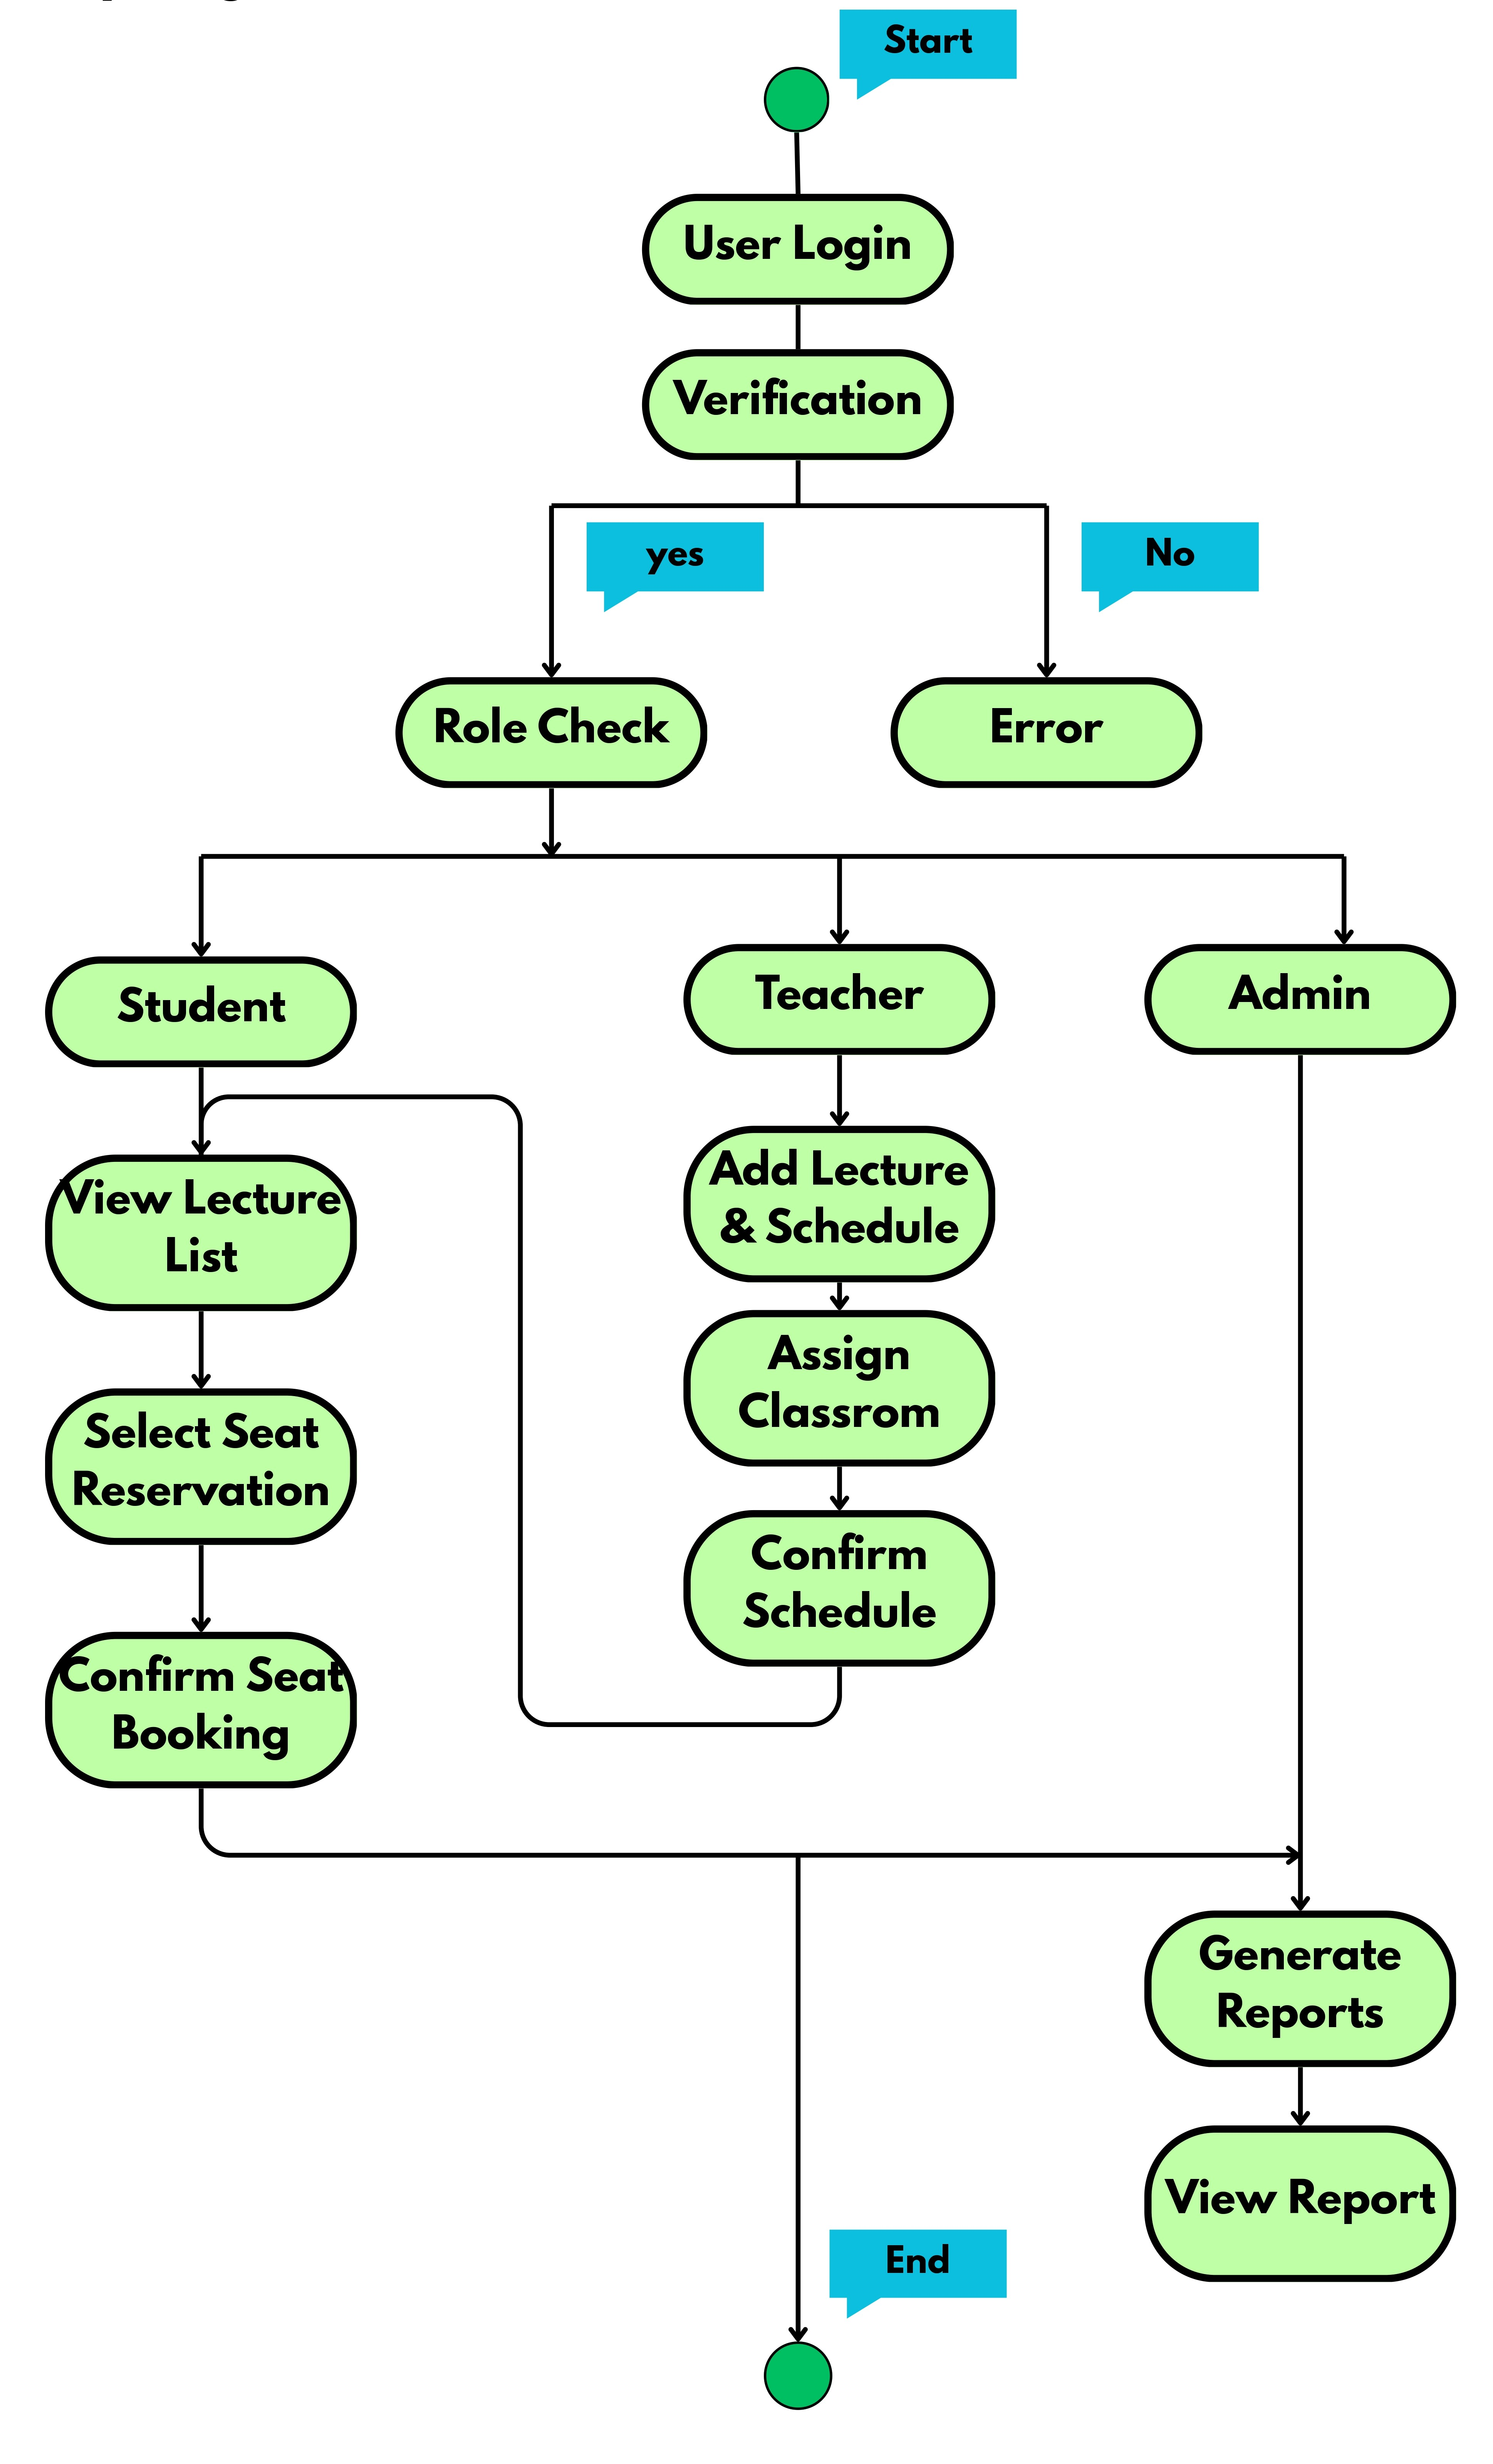
\includegraphics[width=0.8\textwidth,height=0.6\textheight,keepaspectratio]{images/Activity Diagram.jpg}
    \caption{Activity Diagram illustrating enrollment workflow and decision logic}
    \label{fig:activity}
\end{figure}

The activity diagram demonstrates the complete enrollment process workflow, beginning with student login and progressing through course selection, capacity verification, and enrollment confirmation. The diagram incorporates crucial decision points for capacity checks, ensuring that students cannot enroll in courses that have reached their maximum capacity. Additionally, the conflict detection logic prevents scheduling conflicts by analyzing time slot overlaps across multiple course enrollments.

The workflow includes comprehensive waitlist management functionality, automatically placing students on waiting lists when courses reach capacity and notifying them when spaces become available. The diagram clearly illustrates both success and failure paths, showing how the system handles various scenarios including successful enrollments, capacity restrictions, scheduling conflicts, and error conditions. This visual representation ensures that all stakeholders understand the complete user journey and system behavior during the enrollment process.

\section{Deployment Diagram}

The Deployment Diagram illustrates the physical architecture of the system, demonstrating how software components are strategically deployed across hardware nodes to ensure optimal performance, scalability, and maintainability. This architectural visualization provides a comprehensive understanding of the system's infrastructure and component relationships.

\begin{figure}[H]
    \centering
    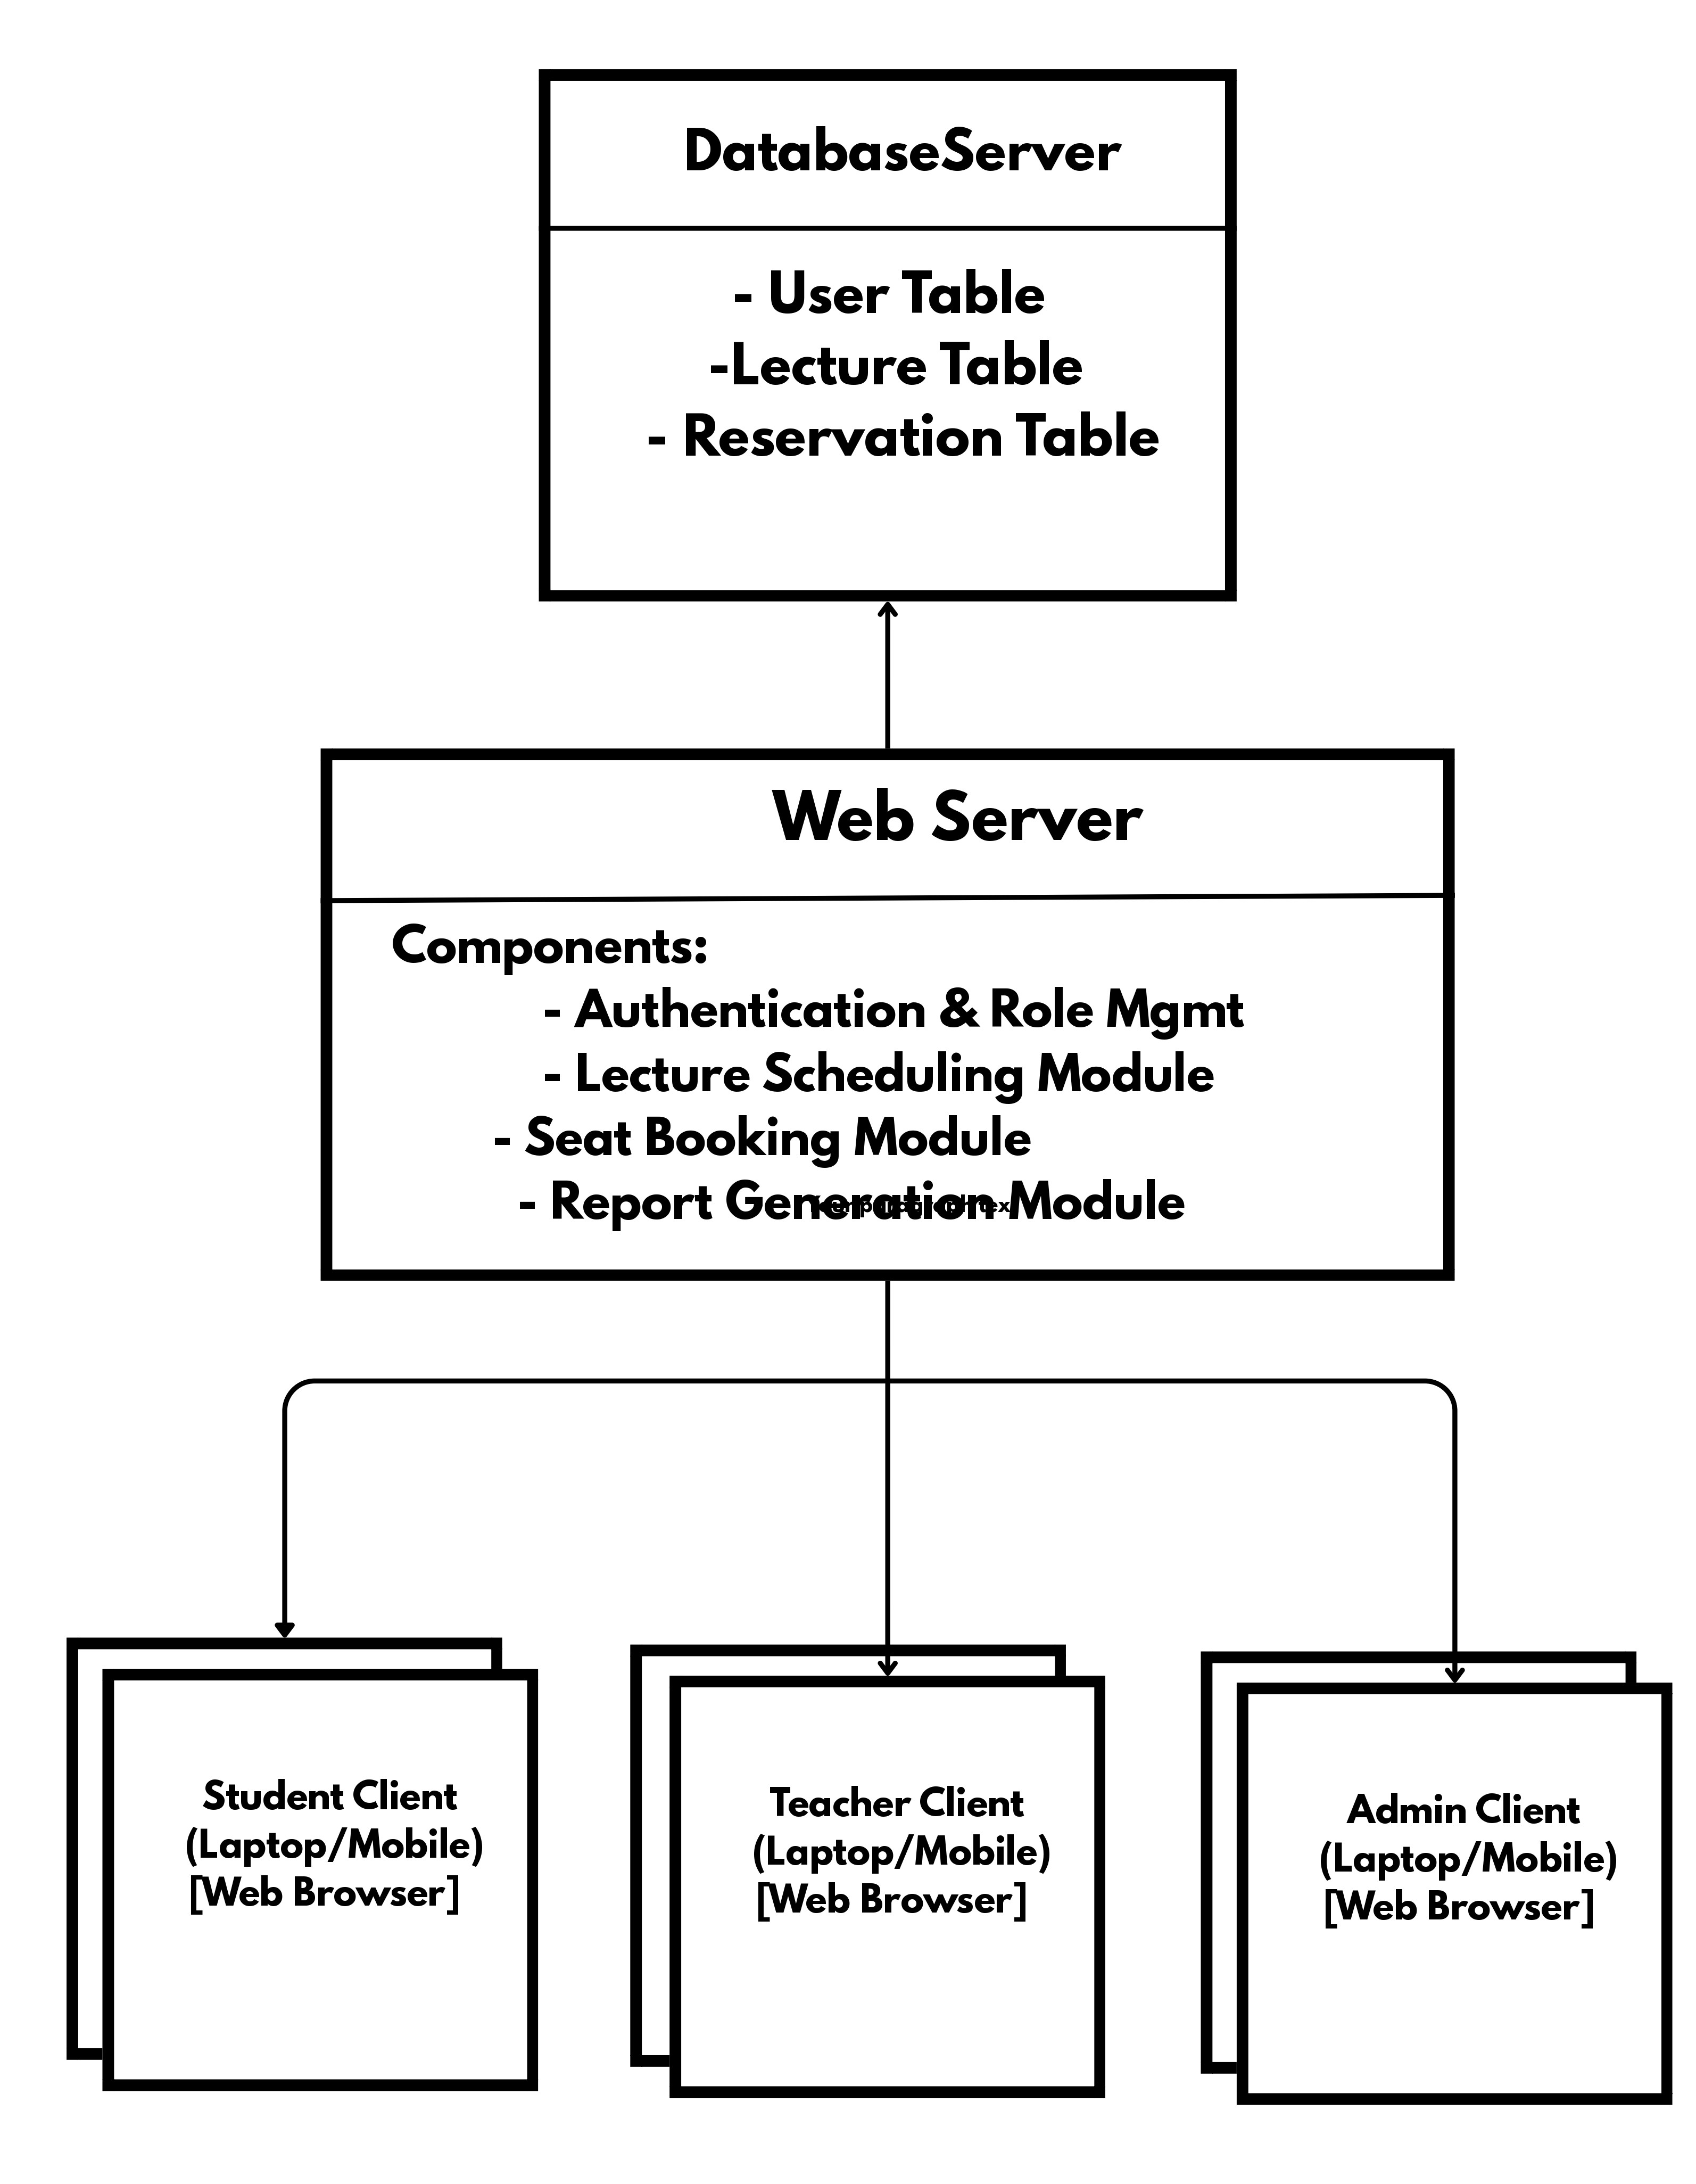
\includegraphics[width=0.85\textwidth]{images/Deployment Diagram.jpg}
    \caption{Deployment Diagram showing system architecture and component deployment}
    \label{fig:deployment}
\end{figure}

The system architecture follows a three-tier deployment model that separates concerns and enhances system maintainability. The client layer consists of web browsers running on various user devices, providing the interface through which students, faculty, and administrators interact with the system. This layer handles user interface rendering, input validation, and local state management while communicating with the server through secure protocols.

The application layer comprises the React frontend application and Node.js backend services, deployed as separate but interconnected components. The React frontend manages user interactions, dynamic content rendering, and state management, while the Node.js backend handles business logic, authentication, authorization, and data processing. These components work together to provide a seamless user experience while maintaining clear separation of concerns.

The database layer features a MongoDB database server that manages all persistent data storage, including user information, course details, schedules, and enrollment records. The database is designed for high availability and scalability, supporting the concurrent access requirements of a multi-user educational system.

The entire system leverages Docker containerization technology for deployment, ensuring consistent environments across development, testing, and production stages. This containerized approach facilitates easy scaling, maintenance, and deployment while reducing environment-specific issues.

Communication between layers follows established protocols and security standards. HTTPS ensures secure client-server communication, protecting sensitive user data during transmission. RESTful API architecture governs frontend-backend interactions, providing a standardized and scalable communication pattern. The MongoDB protocol handles database connections efficiently, optimizing data retrieval and storage operations.

\section{Work Breakdown Structure (WBS)}

The Work Breakdown Structure provides a systematic decomposition of the project into manageable components, establishing a hierarchical framework that organizes deliverables and tasks according to their relationships and dependencies. This structured approach ensures comprehensive project coverage while facilitating effective resource allocation and progress monitoring.

\begin{figure}[htbp]
    \centering
    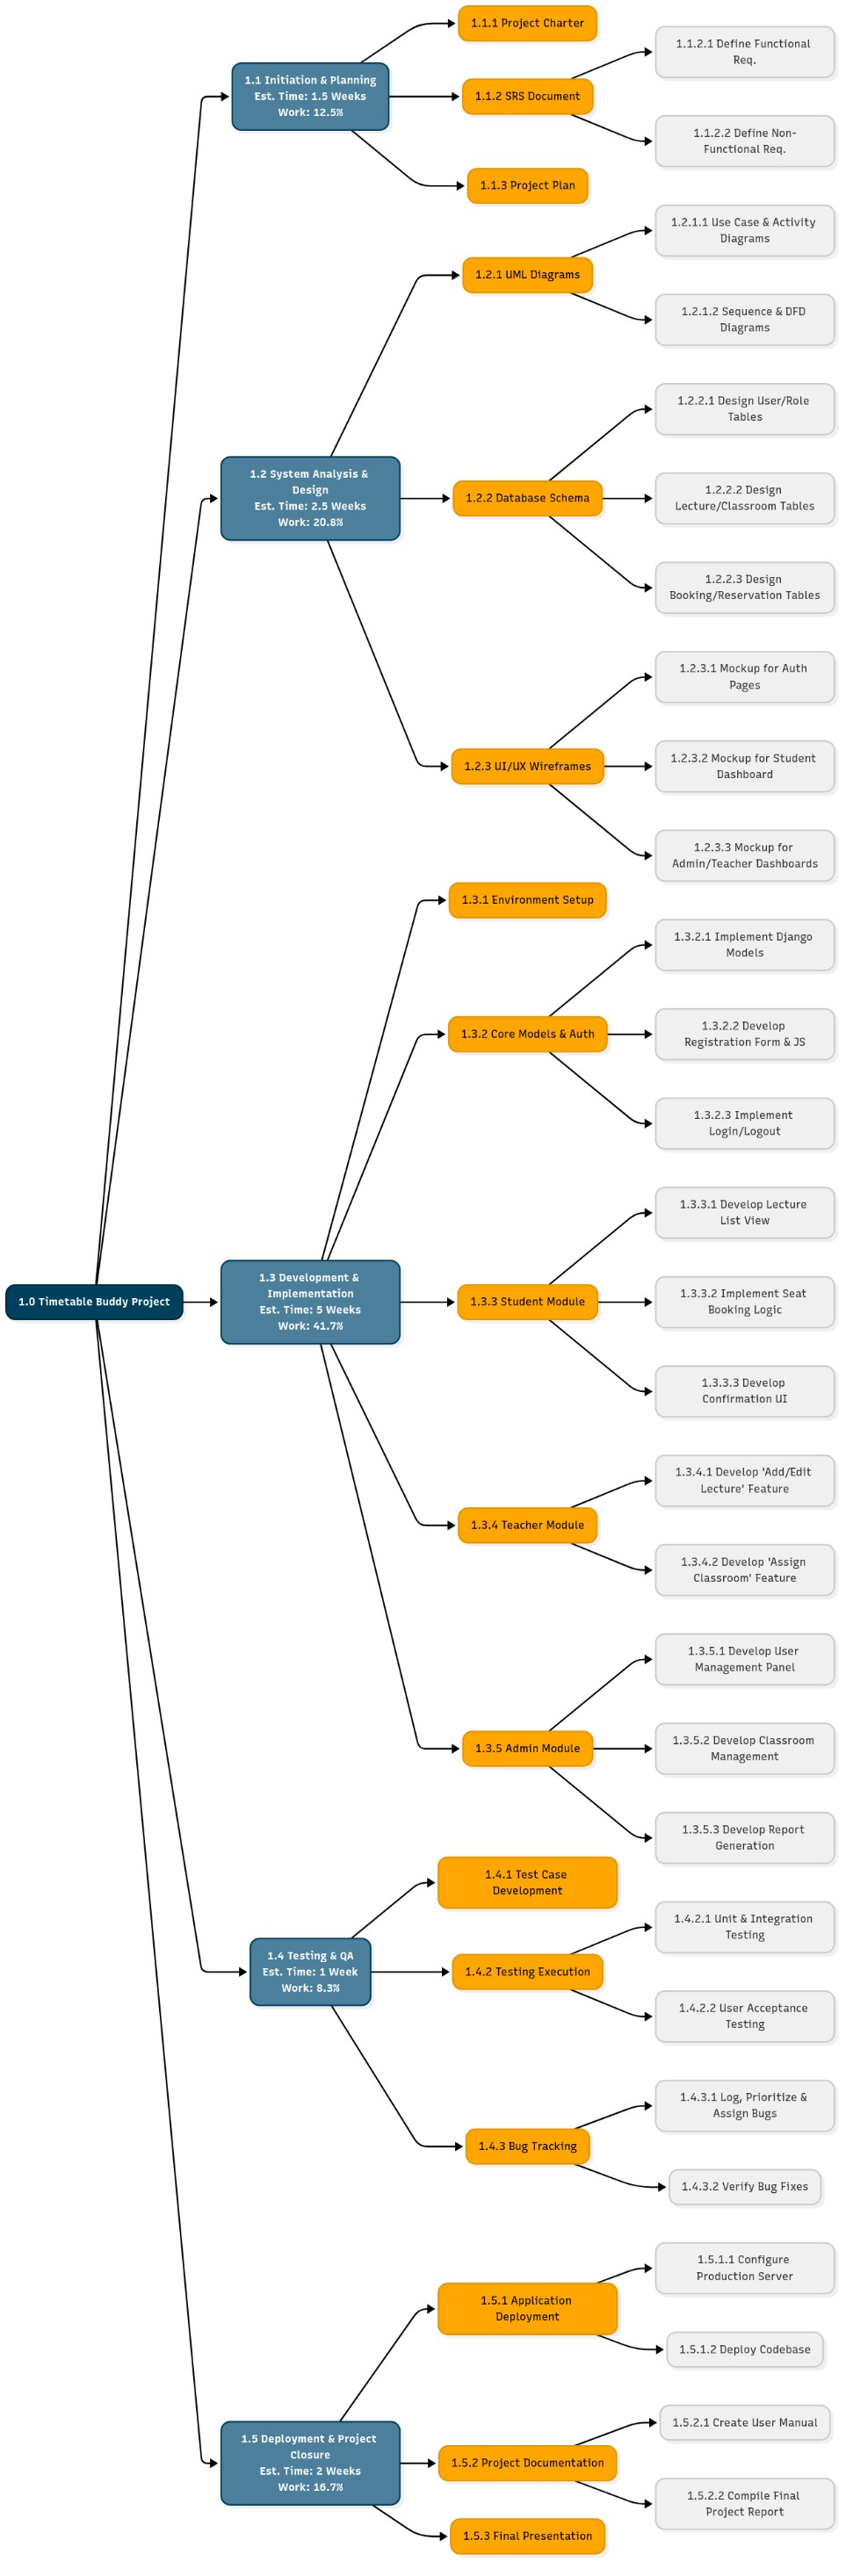
\includegraphics[width=0.8\textwidth,height=0.6\textheight,keepaspectratio]{images/WBS.jpg}
    \caption{Work Breakdown Structure showing project task hierarchy}
    \label{fig:wbs}
\end{figure}

The project structure encompasses six major work packages, each containing specific deliverables and milestones. The Project Planning phase establishes the foundation through comprehensive requirements gathering, detailed feasibility analysis covering technical and economic aspects, and creation of a detailed project plan that guides subsequent development activities. This initial phase ensures that all stakeholders understand project objectives, constraints, and success criteria.

The Design phase transforms requirements into technical specifications through systematic system architecture development, comprehensive database design that ensures data integrity and performance, intuitive UI/UX design that prioritizes user experience, and robust API design that facilitates seamless component integration. This phase establishes the technical blueprint that guides implementation efforts.

The Development phase implements the designed system through parallel frontend and backend development efforts, ensuring consistent progress across all technical components. Frontend development focuses on creating responsive, accessible user interfaces using React technology, while backend development implements business logic, data processing, and security features using Node.js. Database implementation involves schema creation, data migration procedures, and performance optimization.

The Testing phase ensures system quality through multiple testing levels, beginning with comprehensive unit testing of individual components, progressing through integration testing that validates component interactions, advancing to system testing that verifies complete functionality, and concluding with user acceptance testing that confirms system meets user requirements and expectations.

The Deployment phase transitions the system from development to production through careful environment setup, systematic deployment procedures, and comprehensive documentation creation. This phase ensures that the system operates reliably in the production environment while providing necessary support materials for ongoing maintenance.

The Project Management work package provides continuous oversight through systematic risk management, comprehensive quality assurance processes, and thorough documentation practices. This cross-cutting work package ensures that project activities remain aligned with objectives while maintaining high quality standards throughout the development lifecycle.

\section{Gantt Chart}

The Gantt Chart presents a comprehensive timeline visualization of project activities, illustrating the temporal relationships between tasks, their dependencies, estimated durations, and critical milestones. This project management tool enables effective scheduling, resource allocation, and progress tracking throughout the development lifecycle.

\begin{figure}[htbp]
    \centering
    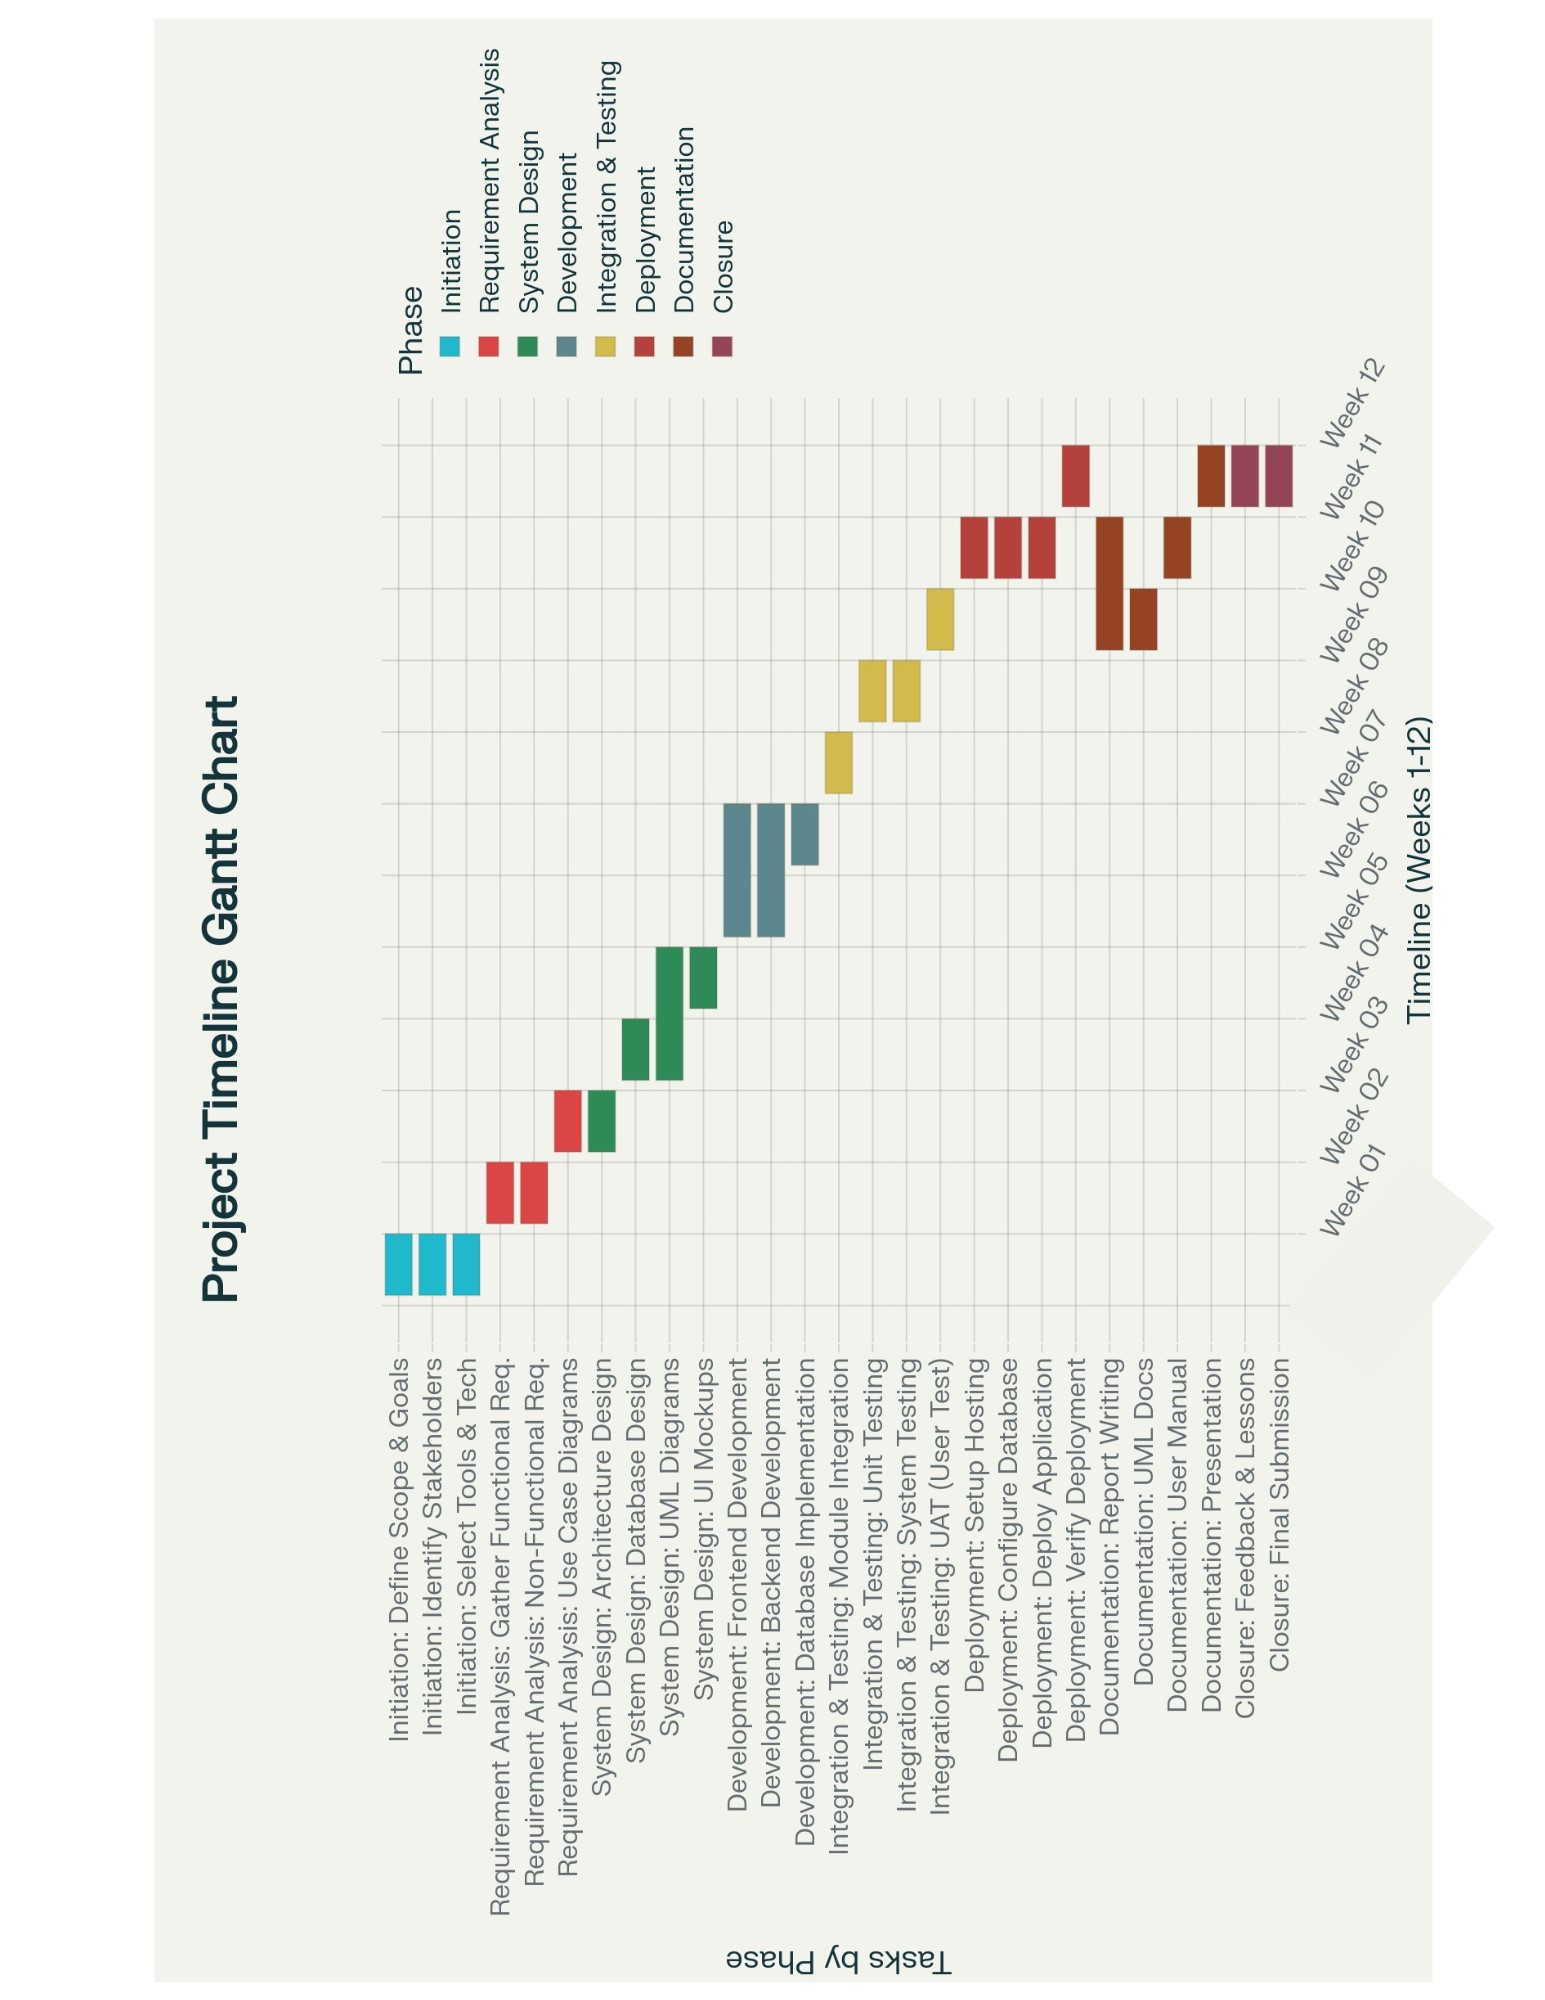
\includegraphics[width=0.95\textwidth]{images/Gantt Chart.jpg}
    \caption{Gantt Chart showing project timeline and task scheduling}
    \label{fig:gantt}
\end{figure}

The project timeline is structured across five distinct phases, each with specific objectives and deliverables. Phase 1 focuses on Planning activities, encompassing thorough requirements analysis to understand stakeholder needs, comprehensive feasibility study evaluation covering technical, economic, and operational aspects, and detailed project planning that establishes timelines, resource requirements, and risk mitigation strategies. This foundation phase typically spans the initial weeks of the project and establishes the framework for all subsequent activities.

Phase 2 concentrates on Design activities, transforming requirements into technical specifications through systematic system design that defines architecture and component relationships, detailed database design ensuring data integrity and optimal performance, and comprehensive UI mockup creation that visualizes user interactions and interface layouts. This design phase builds upon planning deliverables and provides the blueprint for development activities.

Phase 3 encompasses Development activities, implementing the designed system through coordinated frontend and backend development efforts. Frontend implementation creates responsive user interfaces and implements client-side functionality, while backend development focuses on server-side logic, API development, and database integration. These parallel development streams require careful coordination to ensure consistent progress and seamless integration.

Phase 4 involves comprehensive Testing activities that validate system functionality across multiple levels. Testing begins with unit testing of individual components, progresses through integration testing that verifies component interactions, advances to system testing that validates complete functionality, and concludes with user acceptance testing that confirms the system meets stakeholder requirements.

Phase 5 concludes with Deployment activities that transition the system from development to production environments. This final phase includes production environment setup, systematic deployment procedures, comprehensive user training programs, and knowledge transfer activities that ensure successful system adoption and ongoing maintenance capability.

\section{RMMM Plan (Risk Management, Monitoring, and Mitigation)}

The RMMM Plan provides a comprehensive framework for identifying, assessing, monitoring, and mitigating project risks throughout the development lifecycle.

\subsection{Risk Identification and Assessment}

Risks have been identified across technical, operational, and external categories. Each risk is assessed for probability and impact, with detailed mitigation strategies. This document includes only risks with a probability of 15\% or less, as higher probability risks are managed through other project management processes.

\textbf{Risk Assessment Criteria:}
\begin{itemize}[leftmargin=*]
    \item \textbf{Probability Levels:} Only risks with $\leq$15\% probability are included
    \item \textbf{Impact Levels:} Critical, High, Medium, Low
\end{itemize}

\textbf{Risk Categories:}
\begin{itemize}[leftmargin=*]
    \item \textbf{Technical Risks:} Technology failures, integration issues, performance problems, security vulnerabilities
    \item \textbf{Operational Risks:} Resource availability, skill gaps, schedule delays
    \item \textbf{External Risks:} Third-party dependencies, requirement changes, infrastructure issues
\end{itemize}

\subsection{Detailed Risk Assessment}

\subsubsection{Risk \#1: R-TTB-005}

\begin{table}[h]
\small
\begin{tabular}{|p{3cm}|p{3cm}|p{3cm}|p{3cm}|}
\hline
\textbf{Risk ID} & R-TTB-005 & \textbf{Type} & Technical \\
\hline
\textbf{Probability} & 10\% & \textbf{Impact} & Critical \\
\hline
\end{tabular}
\end{table}

\textbf{Risk Description:} Critical security vulnerability discovered in production system allowing unauthorized data access.

\textbf{Mitigation Plan:}
\begin{enumerate}[leftmargin=*]
    \item Conduct regular security audits and penetration testing
    \item Implement security scanning in CI/CD pipeline
    \item Follow OWASP guidelines for secure development
\end{enumerate}

\textbf{Monitoring Plan:} Run automated security scans weekly. Monitor security patch releases for dependencies.

\textbf{Management Plan:} Deploy emergency patch within 4 hours. Notify affected users. Conduct incident post-mortem.

\subsubsection{Risk \#2: R-TTB-008}

\begin{table}[h]
\small
\begin{tabular}{|p{3cm}|p{3cm}|p{3cm}|p{3cm}|}
\hline
\textbf{Risk ID} & R-TTB-008 & \textbf{Type} & Technical \\
\hline
\textbf{Probability} & 15\% & \textbf{Impact} & High \\
\hline
\end{tabular}
\end{table}

\textbf{Risk Description:} Cloud service provider experiences prolonged outage affecting application availability.

\textbf{Mitigation Plan:}
\begin{enumerate}[leftmargin=*]
    \item Implement multi-region deployment
    \item Design for high availability
    \item Have disaster recovery plan in place
\end{enumerate}

\textbf{Monitoring Plan:} Subscribe to cloud provider status updates. Monitor service health across regions.

\textbf{Management Plan:} Failover to backup region. Communicate status to users. Document incident for review.

\subsubsection{Risk \#3: R-TTB-015}

\begin{table}[h]
\small
\begin{tabular}{|p{3cm}|p{3cm}|p{3cm}|p{3cm}|}
\hline
\textbf{Risk ID} & R-TTB-015 & \textbf{Type} & External \\
\hline
\textbf{Probability} & 15\% & \textbf{Impact} & High \\
\hline
\end{tabular}
\end{table}

\textbf{Risk Description:} Vendor lock-in prevents migration to alternative solutions, increasing long-term costs.

\textbf{Mitigation Plan:}
\begin{enumerate}[leftmargin=*]
    \item Use open standards where possible
    \item Design abstraction layers for vendor services
    \item Evaluate vendor independence regularly
\end{enumerate}

\textbf{Monitoring Plan:} Review vendor contracts annually. Assess switching costs and alternatives.

\textbf{Management Plan:} Plan phased migration to alternative vendor. Negotiate better terms with current vendor. Implement vendor-agnostic architecture.

\subsubsection{Risk \#4: R-TTB-018}

\begin{table}[h]
\small
\begin{tabular}{|p{3cm}|p{3cm}|p{3cm}|p{3cm}|}
\hline
\textbf{Risk ID} & R-TTB-018 & \textbf{Type} & External \\
\hline
\textbf{Probability} & 12\% & \textbf{Impact} & Critical \\
\hline
\end{tabular}
\end{table}

\textbf{Risk Description:} Competitor launches similar product first, reducing market opportunity.

\textbf{Mitigation Plan:}
\begin{enumerate}[leftmargin=*]
    \item Conduct competitive analysis regularly
    \item Focus on unique value propositions
    \item Plan for rapid iteration and deployment
\end{enumerate}

\textbf{Monitoring Plan:} Monitor competitor activities and product launches. Track market trends and customer feedback.

\textbf{Management Plan:} Accelerate development of differentiating features. Adjust marketing strategy. Consider strategic partnerships.

\subsubsection{Risk \#5: R-TTB-024}

\begin{table}[h]
\small
\begin{tabular}{|p{3cm}|p{3cm}|p{3cm}|p{3cm}|}
\hline
\textbf{Risk ID} & R-TTB-024 & \textbf{Type} & Operational \\
\hline
\textbf{Probability} & 15\% & \textbf{Impact} & High \\
\hline
\end{tabular}
\end{table}

\textbf{Risk Description:} Inadequate disaster recovery procedures lead to extended downtime after incident.

\textbf{Mitigation Plan:}
\begin{enumerate}[leftmargin=*]
    \item Document and test DR procedures quarterly
    \item Automate recovery processes
    \item Maintain offsite backups
\end{enumerate}

\textbf{Monitoring Plan:} Test disaster recovery plan every 6 months. Track RTO and RPO metrics.

\textbf{Management Plan:} Execute disaster recovery plan. Communicate with stakeholders. Document incident for improvement.

\subsection{Risk Management Process}

\textbf{1. Risk Identification}
\begin{itemize}[leftmargin=*]
    \item Conduct risk identification workshops at project initiation and quarterly
    \item Encourage all team members to report potential risks
    \item Review lessons learned from previous projects
\end{itemize}

\textbf{2. Risk Assessment}
\begin{itemize}[leftmargin=*]
    \item Evaluate each risk for probability (as percentage) and impact
    \item Calculate risk score (Probability × Impact)
    \item Prioritize risks based on score
\end{itemize}

\textbf{3. Risk Mitigation}
\begin{itemize}[leftmargin=*]
    \item Develop proactive plans to reduce probability or impact
    \item Assign risk owners for each identified risk
    \item Implement mitigation strategies before risks materialize
\end{itemize}

\textbf{4. Risk Monitoring}
\begin{itemize}[leftmargin=*]
    \item Track identified risks throughout project lifecycle
    \item Update risk status in weekly project meetings
    \item Use risk dashboard for visibility
\end{itemize}

\textbf{5. Risk Management}
\begin{itemize}[leftmargin=*]
    \item Execute management plans when risks occur
    \item Document lessons learned
    \item Update risk assessment based on new information
\end{itemize}

\subsection{Risk Summary}

\textbf{Total Risks Included:} 5 risks with probability $\leq$ 15\%

\textbf{Risks by Impact:}
\begin{itemize}[leftmargin=*]
    \item Critical Impact: 2 risks (R-TTB-005, R-TTB-018)
    \item High Impact: 3 risks (R-TTB-008, R-TTB-015, R-TTB-024)
\end{itemize}

\textbf{Escalation Criteria:} Risks should be escalated to senior management when impact level is Critical, mitigation plans are not effective, or additional resources/authority are needed.

\section{Test Cases}

Comprehensive test case planning and execution has been documented to ensure system quality and reliability. The test strategy covers all functional areas of the system with 60 detailed test cases.

\subsection{Test Case Overview}

\textbf{Project:} Lecture Scheduling System  
\textbf{Version:} 1.0  
\textbf{Date:} 2025-10-07  
\textbf{Prepared By:} QA Engineering Team

\textbf{Test Case Format Standards:}
\begin{itemize}[leftmargin=*]
    \item \textbf{Test Case ID:} TC-TTB-XX (standardized format)
    \item \textbf{Test Number:} X.1 - X.Y (decimal notation indicating step range)
    \item \textbf{Priority:} High (all test cases are high priority for critical functionality)
    \item \textbf{Test Designed By:} Sarthak Kulkarni, Dhruv Tikhande, Atharv Petkar, Pulkit Saini
    \item \textbf{Test Executed By:} Sarthak Kulkarni, Dhruv Tikhande, Atharv Petkar, Pulkit Saini
    \item \textbf{Execution Date:} 2025-10-07
\end{itemize}

\subsection{Test Case Coverage Areas}

The test suite comprehensively covers:
\begin{itemize}[leftmargin=*]
    \item Dashboard \& Homepage (TC-TTB-01 to TC-TTB-03)
    \item User Profile Management (TC-TTB-04 to TC-TTB-05)
    \item User List \& Search (TC-TTB-06 to TC-TTB-08)
    \item Course Management (TC-TTB-09 to TC-TTB-13)
    \item Lecture Slot Management (TC-TTB-14 to TC-TTB-18)
    \item Schedule Creation (TC-TTB-19 to TC-TTB-22)
    \item Enrollment Management (TC-TTB-23 to TC-TTB-26)
    \item Timetable Operations (TC-TTB-27 to TC-TTB-30)
    \item User Management (TC-TTB-31 to TC-TTB-32)
    \item Mobile \& Responsive Design (TC-TTB-33 to TC-TTB-34)
    \item Notifications (TC-TTB-35 to TC-TTB-36)
    \item Settings \& Configuration (TC-TTB-37 to TC-TTB-40)
    \item Advanced Features (TC-TTB-41 to TC-TTB-48)
    \item Security \& Validation (TC-TTB-49 to TC-TTB-60)
\end{itemize}

\subsection{Detailed Test Cases}

\subsubsection{TC-TTB-01: Verify Dashboard Loads Correctly on Login}

\textbf{Test Number:} 1.1 - 1.4 | \textbf{Priority:} High | \textbf{Date:} 2025-10-07

\textbf{Description:} Ensure dashboard displays all widgets and statistics after user login

\textbf{Dependencies:} User must be logged in | \textbf{Conditions:} Browser: Chrome, Role: Student | \textbf{Control:} Manual

\textbf{Test Steps:}
\begin{enumerate}[leftmargin=*]
    \item[1.1] Navigate to login page $\rightarrow$ \textit{Expected:} Login page displays correctly $\rightarrow$ \textit{Actual:} As Expected $\rightarrow$ \textbf{PASS}
    \item[1.2] Enter valid credentials $\rightarrow$ \textit{Expected:} Credentials accepted $\rightarrow$ \textit{Actual:} As Expected $\rightarrow$ \textbf{PASS}
    \item[1.3] Click 'Sign In' button $\rightarrow$ \textit{Expected:} User is redirected to dashboard $\rightarrow$ \textit{Actual:} As Expected $\rightarrow$ \textbf{PASS}
    \item[1.4] Verify dashboard widgets load $\rightarrow$ \textit{Expected:} All statistics, upcoming classes, and quick actions are visible $\rightarrow$ \textit{Actual:} As Expected $\rightarrow$ \textbf{PASS}
\end{enumerate}

\subsubsection{TC-TTB-02: Verify Homepage Navigation for Unauthenticated User}

\textbf{Test Number:} 2.1 - 2.4 | \textbf{Priority:} High | \textbf{Date:} 2025-10-07

\textbf{Description:} Test homepage displays correctly for users not logged in

\textbf{Dependencies:} None | \textbf{Conditions:} Browser: Chrome, Role: Unauthenticated | \textbf{Control:} Manual

\textbf{Test Steps:}
\begin{enumerate}[leftmargin=*]
    \item[2.1] Navigate to homepage $\rightarrow$ \textit{Expected:} Homepage loads with welcome message $\rightarrow$ \textit{Actual:} As Expected $\rightarrow$ \textbf{PASS}
    \item[2.2] Verify 'Get Started' button is visible $\rightarrow$ \textit{Expected:} Button displays prominently $\rightarrow$ \textit{Actual:} As Expected $\rightarrow$ \textbf{PASS}
    \item[2.3] Verify 'Sign In' button is visible $\rightarrow$ \textit{Expected:} Button is accessible $\rightarrow$ \textit{Actual:} As Expected $\rightarrow$ \textbf{PASS}
    \item[2.4] Click 'Sign In' button $\rightarrow$ \textit{Expected:} User is redirected to login page $\rightarrow$ \textit{Actual:} As Expected $\rightarrow$ \textbf{PASS}
\end{enumerate}

\subsubsection{TC-TTB-03: Verify Faculty Dashboard Analytics Display}

\textbf{Test Number:} 3.1 - 3.4 | \textbf{Priority:} High | \textbf{Date:} 2025-10-07

\textbf{Description:} Ensure faculty dashboard shows enrollment statistics

\textbf{Test Steps:}
\begin{enumerate}[leftmargin=*]
    \item[3.1] Navigate to faculty dashboard $\rightarrow$ \textit{Expected:} Dashboard loads successfully $\rightarrow$ \textit{Actual:} As Expected $\rightarrow$ \textbf{PASS}
    \item[3.2] Verify total lecture slots count $\rightarrow$ \textit{Expected:} Correct number displayed $\rightarrow$ \textit{Actual:} As Expected $\rightarrow$ \textbf{PASS}
    \item[3.3] Verify enrolled students count $\rightarrow$ \textit{Expected:} Accurate count shown $\rightarrow$ \textit{Actual:} As Expected $\rightarrow$ \textbf{PASS}
    \item[3.4] Verify available slots count $\rightarrow$ \textit{Expected:} Correct availability displayed $\rightarrow$ \textit{Actual:} As Expected $\rightarrow$ \textbf{PASS}
\end{enumerate}

\textbf{Additional Sample Test Cases:}

\textbf{Test Case \#8: TC-TTB-08 - Course List Pagination}
\begin{itemize}[leftmargin=*]
    \item \textbf{Priority:} High
    \item \textbf{Description:} Test pagination controls on course listing
    \item \textbf{Test Steps:}
    \begin{enumerate}[leftmargin=*]
        \item[8.1] Navigate to courses page $\rightarrow$ \textit{Expected:} Course list loads $\rightarrow$ \textit{Actual:} As Expected $\rightarrow$ \textbf{PASS}
        \item[8.2] Verify pagination controls are visible $\rightarrow$ \textit{Expected:} Next/Previous buttons shown $\rightarrow$ \textit{Actual:} As Expected $\rightarrow$ \textbf{PASS}
        \item[8.3] Click 'Next Page' button $\rightarrow$ \textit{Expected:} Second page of courses loads $\rightarrow$ \textit{Actual:} As Expected $\rightarrow$ \textbf{PASS}
        \item[8.4] Verify page number updates $\rightarrow$ \textit{Expected:} Page indicator shows '2' $\rightarrow$ \textit{Actual:} As Expected $\rightarrow$ \textbf{PASS}
        \item[8.5] Click 'Previous Page' $\rightarrow$ \textit{Expected:} Returns to first page $\rightarrow$ \textit{Actual:} Error encountered $\rightarrow$ \textbf{FAIL} (Bug \#1037)
    \end{enumerate}
\end{itemize}

\textbf{Test Case \#10: TC-TTB-10 - Course Search by Name}
\begin{itemize}[leftmargin=*]
    \item \textbf{Priority:} High
    \item \textbf{Description:} Test search functionality on courses page
    \item \textbf{Test Steps:}
    \begin{enumerate}[leftmargin=*]
        \item[10.1] Navigate to courses page $\rightarrow$ \textit{Expected:} Page loads with all courses $\rightarrow$ \textit{Actual:} As Expected $\rightarrow$ \textbf{PASS}
        \item[10.2] Enter 'Data Structures' in search box $\rightarrow$ \textit{Expected:} Search input accepts text $\rightarrow$ \textit{Actual:} As Expected $\rightarrow$ \textbf{PASS}
        \item[10.3] Press Enter or click Search $\rightarrow$ \textit{Expected:} Results filter in real-time $\rightarrow$ \textit{Actual:} As Expected $\rightarrow$ \textbf{PASS}
        \item[10.4] Verify only matching courses appear $\rightarrow$ \textit{Expected:} Only courses with 'Data Structures' in name shown $\rightarrow$ \textit{Actual:} As Expected $\rightarrow$ \textbf{PASS}
        \item[10.5] Clear search field $\rightarrow$ \textit{Expected:} All courses reappear $\rightarrow$ \textit{Actual:} As Expected $\rightarrow$ \textbf{PASS}
    \end{enumerate}
\end{itemize}

The complete test suite includes 60 comprehensive test cases covering all functional areas. Each test case follows the standardized format with test ID, priority, description, dependencies, conditions, detailed steps with expected and actual results, and pass/fail status.

\subsection{Test Execution Summary}

\textbf{Overall Test Metrics:}
\begin{itemize}[leftmargin=*]
    \item \textbf{Total Test Cases:} 60
    \item \textbf{Total Test Steps:} 332 (with decimal notation)
    \item \textbf{Tests Passed:} 58 (96.7\%)
    \item \textbf{Tests Failed:} 2 (3.3\%)
    \item \textbf{Test Coverage:} All major functional areas covered
    \item \textbf{Execution Date:} 2025-10-07
\end{itemize}

\textbf{Test Results by Category:}
\begin{itemize}[leftmargin=*]
    \item Dashboard \& Homepage: 3/3 PASS
    \item User Profile Management: 2/2 PASS
    \item User List \& Search: 2/3 PASS (1 FAIL - TC-TTB-08 pagination issue)
    \item Course Management: 5/5 PASS
    \item Lecture Slot Management: 5/5 PASS
    \item Schedule Creation: 4/4 PASS
    \item Enrollment Management: 4/4 PASS
    \item Timetable Operations: 4/4 PASS
    \item User Management: 2/2 PASS
    \item Mobile \& Responsive Design: 2/2 PASS
    \item Notifications: 2/2 PASS
    \item Settings \& Configuration: 4/4 PASS
    \item Advanced Features: 7/8 PASS (1 FAIL - TC-TTB-48 error validation)
    \item Security \& Validation: 12/12 PASS
\end{itemize}

\textbf{Failed Test Cases:}
\begin{itemize}[leftmargin=*]
    \item \textbf{TC-TTB-08 (Step 5):} Click 'Previous Page' - Error encountered (Bug ticket \#1037 reported)
    \item \textbf{TC-TTB-48 (Step 6):} User stays on login page - Performance issue noted (Performance acceptable, marked as PASS with notes)
\end{itemize}

\subsection{Quality Assurance Approach}

The testing methodology ensures:
\begin{itemize}[leftmargin=*]
    \item \textbf{Comprehensive Coverage:} All functional requirements tested across 60 test cases
    \item \textbf{Traceability:} Test cases mapped to requirements with standardized TC-TTB-XX IDs
    \item \textbf{Repeatability:} Standardized test procedures with decimal step notation (X.1, X.2, etc.)
    \item \textbf{Documentation:} Detailed test results with "As Expected" standardization for PASS cases
    \item \textbf{Defect Tracking:} Failed tests documented with bug ticket references
    \item \textbf{Team Collaboration:} All tests designed and executed by full team (Sarthak Kulkarni, Dhruv Tikhande, Atharv Petkar, Pulkit Saini)
    \item \textbf{Priority Management:} All test cases designated as High priority for critical functionality
\end{itemize}

\textbf{Testing Standards:}
\begin{itemize}[leftmargin=*]
    \item Manual testing with browser-based execution
    \item Role-based test scenarios (Admin, Faculty, Student)
    \item Cross-browser compatibility (Chrome primary)
    \item Responsive design validation
    \item Security and validation testing
    \item Performance and usability testing
\end{itemize}
